\chapter{\label{chapter:PropagatorStates}The State Vector and State Management}
\chapauthor{Darrel J. Conway}{Thinking Systems, Inc.}

GMAT supplies a class, the GmatState, which provides a low level container for mission related
state information manipulated by the system during a simulation.  The GmatState is populated with
data from the objects in GMAT's current model so that the code that implements the processes in the
simulation can act on the data in a generic fashion.  The synchronization between the data that
is manipulated and the objects that supply these data is handled by classes derived from the
StateManager class.  These interactions are described at a high level in this chapter.  Specific
uses of the state vector and managers can be found in the chapters describing propagation
(Chapter~\ref{chapter:PropagatorOverview}) and orbit determination
(Chapter~\ref{chapter:Estimation}).

\section{Design Motivation and Overview}

The combination of one or more GmatState objects and one or more associated StateManagers as
implemented in GMAT follows the Mediator design pattern.  The GmatState acts as an object
that accumulates data from the elements of GMAT's mission into a format that can be used by the
algorithms that manipulate these data to run a mission.  Once these algorithms complete their work,
the changed data in the GmatState object is then passed back to the objects representing physical
entities in the model.  The coordination of the GmatState with the objects providing the state data
is handled by an instance of a class derived from the StateManager class.

GMAT uses this intermediary to keep the propagation and estimation processes as generic as
possible.  In GMAT, the propagation algorithms work by advancing an arbitrarily sized vector of
numbers over time.  Knowledge about the way these numbers evolve is all predefined when the
propagators are set up prior to the actual evolution.  This predefined setup and subsequent
application of the propagation algorithm streamlines the process of changing the state of GMAT's
objects as the model epoch changes.  It also makes the definition of the propagation vector
flexible and extensible.  New elements that need to evolve over time can be added to GMAT's
propagation subsystem by defining an ID for the new propagation type, supplying the corresponding
evolution providers (for instance, a PhysicalModel defining ordinary differential equations used
to integrate the new element), and changes making this new element visible to the propagation
enabled commands.

Similarly, in GMAT estimation is constructed to apply an estimation algorithm to an arbitrarily
sized vector of numbers.  The connection between the state vector used in the estimation process and
the objects defined in GMAT's mission is made when the estimation subsystem is initialized.  The
synchronization of data between the estimation vector and the mission obects is managed by an
instance of a class derived from the StateManager class.  This abstraction of the estimation state
vector from the mission defined objects is used to keep the estiamtion subsystem extensible and
flexible in the same way as is provided for the propagation subsystem.

An added feature of this design is that any other algorithms that work on a vector of numbers
and an associated epoch can use GMAT's objects to build this generic data set simply by deriving a
new StateManager appropriate to the algorithm and using that StateManager to handle the data
interchange between the state vector and the associated GMAT objects.  Implementors that need such
new capablities in GMAT need only study the patterns implemented in the estimation and propagation
subsystems in order gain insight into how to extend GMAT for these new capabilities.

\subsection[A Propagation State Example]{An Example: State and State Management in Propagation}

You can see an example of this mediation\footnote{A more detailed look at the objects and
interactions in this example can be found in Section~\ref{section:PropagationExample}.  This
section is intended to illustrate how the objects, state and state manager operate in teh context
of the example mission.} in GMAT's propagation subsystem. Consider a mission consisting of two
spacecraft that are propagated for a day using a Runge-Kutta integrator and a force model consisting
of a 4x4 geopotential model, point mass effects from the Sun and Moon, solar radiation pressure, and
atmospheric drag modeled using the MSISE-90 atmosphere model.  In GMAT, the user configures four
objects to model this system: two spacecraft, an ODEModel that holds the force model, and a
Runge-Kutta integrator.  The mission control sequence that uses these objects is a single Propagate
command.  Ignoring the details of the object configuration, the setup for this mission can be
scripted:

\begin{quote}
\texttt{Create Spacecraft sat1 sat2\\
\\
Create ForceModel fm\\
Create Propagator prop\\
prop.FM = fm\\
\\
\% The Mission Control Sequence\\
Propagate prop(sat1, sat2) \{sat1.ElapsedDays = 1.0\}}
\end{quote}

\noindent From the perspective of the state vetor and manager, the behavior required by this
scripting can be broken into four phases followed by GMAT's propagation subsystem when running a
mission: (1) Script Parsing, (2) Initialization in the Sandbox, (3) Final Preparation before
propagation, and (4) Propagation.  (The fifth phase in the life of a propagation enabled
command, command finalization, does not have a direct affect on the state and state manager
elements in this script.)  The following paragraphs provide an overview of how state and the state
manager behave in each of these phases.

\begin{enumerate}
\item \textbf{Script Parsing}  During script parsing, all four of the resources in the script --
two spacecraft, the force model, and the PropSetup -- are created and placed in GMAT's global
configuration.  Three of these resources contain GmatState members: each Spacecraft uses a
GmatState to hold the orbital state and epoch information, and the ODEModel (defined by the
ForceModel line) contains a GmatState pointer, which is not yet initialized.  The PropSetup defined
by the Propagator line contains an instance of the PropagationStateManager class, a subclass of
StateManager.  That PropagationStateManager, in turn, contains a GmatState object that will be used
by the PropSetup's propagator as the container for the raw data that gets propagated.

\item \textbf{Initialization}  When a run is started that uses these objects, GMAT clones each
object into the Sandbox used for the run.  That places a copy of the object, including each member
GmatState and PropagationStateManager, into the Sandbox's object store.  The objects in the object
store are then initialized.  As part of this process, object references that won't change because
of actions performed in the Mission Control Sequence are set.  For this script, the ODEModel
containing the force model is passed into PropSetup during this initialization.

Once the objects have been initialized, the Mission Control Sequence performs its initialization.
Each command is passed the Sandbox object stores (that is, the local object map and the global
object store) and the local solar system.  Each command is then issued an instttruction to perform
its initialization.  For our example, the only command in the Mission Control Sequence is a
Propagate command.  On initialization, this command retrieves the PropSetup it needs and clones it
for use by teh command.  This cloning makes copies of the Propagator and (if set) the ODEModel.
The Propagate command then locates each of teh other referenced objects it uses.  It passes the
objects calling for propagation (in this case, sat1 and sat2) into the PropagationStateManager
associated with the PropSetup.  Once these objects have been set, the command initializes the
PropagationStateManager by calling the methods that build the state vector and associate the
objects with the elements of that vector.  The resulting state is passed to the local ODEModel,
completing the part of the command initialization concerned with the state vector and state manager.

\item \textbf{Preparation for Propagation}  The final piece of initialization that occurs prior to
propagation captures all of the data from the objects.

\item \textbf{Propagation}
\end{enumerate}



%\section{\label{section:MissionStateOverview}The Mission State}

% The current values of spacecraft data, the state transition matrix, and other elements that evolve
% in GMAT's model are held, in the propagation subsystem, in the mission state\footnote{Here -- and
% throughout this chapter -- the term ``mission state'' and the word ``state'' represent this
% collection of data elements, unless otherwise specified.  Other chapters in the architectural
% specification may use the word ``state'' for different purposes -- for example, the Solver classes
% all function through finite state machines, where the current location of the system in the
% solution process is assigned a specific status, called a state, and move from one of these
% enumerated stated to another as the solution process is executed.}.  GMAT's mission state can be
% further decomposed into static components, components that evolve through numerical integration,
% components that have analytic evolution operators, and components that are modeled over time using
% stochastic models.
%
% \section{Classes Supporting the Mission State}
%
% The mission state data is culled from the objects that make use of the data contained in the
%state,
% and passed into the elements that the propagators use to calculate the state evolution.  As an
% example, each Spacecraft object manages data representing the position and velocity of that
% particular Spacecraft.  When GMAT needs to model the motion of that spacecraft, it gathers the
% epoch and corresponding position and velocity information in a mission state, and passes that
% mission state to the evolution operator so that the motion associated with the change of epoch can
% be calculated.  A more complete example of this process is presented in
% Section~\ref{section:IntegratorExample}.

\section{The GmatState Class}

% The MissionState class plays two roles in GMAT.  It acts as a container class that takes pointers
% to the objects that supply state data, providing a central location for the state data for mission
% elements that use it.  It also supplies the accumulated state data to those elements in the form
% that they need in order to process it and take actions, and routes any resulting changes in state
% to the objects that receive those changes.
%
% The MissionState class collects data into vectors used by the propagators.  These vectors are
% constructed based on the needs of the propagator, and
%
% GMAT's Numerical Integrators

\subsection{MissionState Attributes}

\begin{itemize}
\item\textbf{Real epoch} The epoch of the state data managed by the MissionState.  GMAT requires
that all such state data in a MissionState use the same epoch.
\item\textbf{ObjectArray dataSource} The vector of objects that are propagated
\item\textbf{std::vector<PropMode> propModes} The propagation mode for each object that is
propagated.
\item\textbf{Integer dimension} Total number of elements that are propagated
\item\textbf{PropVector thePropVector} The state data to be propagated
\end{itemize}

\subsubsection{MissionState Methods}

\begin{itemize}
\item\textbf{bool AddSource(GmatBase* src, PropMode mode, ElementType type, Integer elementId)}
Registers an object as a data provider with the MissionState.  The mode parameter identifies the
type of propagation desired: analytic, numerically integrated, or from an ephemeris source.  The
type parameter identified the kind of element that is propagated.  The elementId parameter is the ID
for the start of the data that is propagated.  All propagated data must be accessible using the
generic access methods defined for GmatBase objects, so that the elementId can be used to access
these data.
\item\textbf{bool Initialize()}  Performs preliminary setup of the PropVector prior to propagation.
\item \textbf{bool PrepareToPropagate()}  Completes pre-propagation setup.
\end{itemize}

\section{\label{section:propVector}The PropVector Class}

%The propVector component of the MissionState is a Real array of data sized to match the data vector
%needed by GMAT's numerical integrators for propagation.  The propVector is constructed by the
%MisisonState when the PrepareToPropagate methos if executed by the command that controls the
%propagation.  Figure~\ref{figure:PropVectorComponents} shows a representative layout for a
%propVector.

Figure~\ref{figure:PropVectorComponents} shows a representative layout of the data in a PropVector
for a single spacecraft.  The vector displayed here is the PropVector used by a numerical
integrator that is modeling the evolution of the spacecraft's trajectory, state transition matrix,
and attitude during a finite burn maneuver.  When a MissionState object assembles a PropVector, it
follows a set of ordering rules designed to make the data in the PropVector fall in a specific
order so that access from the propagators is simplified.  The general order, as shown in this
example, is to place trajectory data first in the vector, followed by associated matrices that
evolve along with the trajectory, then attitude data followed by associated attitde matrices, then
user defined elements, and finally transitory elements like mass, which only changes (through
propagation) during maneuvers.

\begin{figure}[htb]
\begin{center}
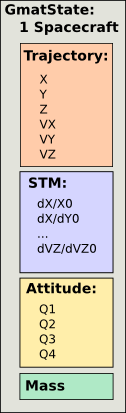
\includegraphics[63,207]{Images/PropVectorComponents.png}
\caption{\label{figure:PropVectorComponents}Representative Elements of a PropVector}
\end{center}
\end{figure}

This ordering can be seen more explicitly in Figure~\ref{figure:ThreeSatPropVector}.  The
PropVector shown in this figure is a vector constructed for three spacecraft, where the mission
needs to propagate the trajectory, state transition matrix, and attitude for all three while
maneuvering all three simultaneously.

\begin{figure}[htb]
\begin{center}
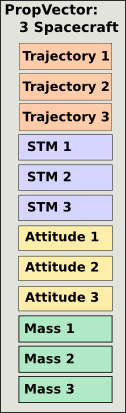
\includegraphics[63,207]{Images/ThreeSatPropVector.png}
\caption{\label{figure:ThreeSatPropVector}Element Arrangement of a PropVector for Three
Spacecraft}
\end{center}
\end{figure}

Figure~\ref{figure:SelectPropVector} shown another example, where the propagation need not
integrate every element of all of the spacecraft.  In this example, the trajector is integrated for
all three spacecraft.  The state transition matrix is only propagated for the first and third
spacecraft, the attitude is propagated for the second, and the first spacecraft is depleting mass
during a maneuver.

\begin{figure}[htb]
\begin{center}
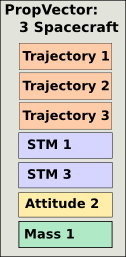
\includegraphics[63,129]{Images/ThreeSatActivePropVector.png}
\caption{\label{figure:SelectPropVector}Three Spacecraft Arrangement for Select
Propagation}
\end{center}
\end{figure}

Figure~\ref{figure:AttitudePropVector} \textbf{This figure needs updating to include the second
PropVector for the trajectory piece} shows a mixed mode propagation, where the trajectory for our
three spacecraft is propagated using a precalculated, ephemeris based propagator and the attitude is
propagated numerically.

\begin{figure}[htb]
\begin{center}
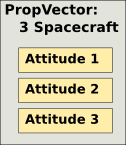
\includegraphics[63,73]{Images/ThreeSatAttitudePropVector.png}
\caption{\label{figure:AttitudePropVector}PropVector for Attitude Only Propagation on Three
Spacecraft}
\end{center}
\end{figure}


\subsection{Enumerations used in State Management}

The MissionState uses several enumerations used to identify propagation components efficiently.
This section describes each of these enumerations.

\paragraph{PropMode}  The PropMode enumeration identifies the type of propagation used with a given
set of state elements.

\begin{itemize}
\item \textbf{ANALYTIC\_PROP}
\item \textbf{INTEGRATE}
\item \textbf{PRECALCULATED\_PROP}
\end{itemize}

\paragraph{ElementType}  The ElementType enumeration identifies the kind of component contained in
a PropVector

\begin{itemize}
\item \textbf{CARTESIAN\_START}
\item \textbf{CARTESIAN}
\item \textbf{EQUINOCTIAL\_START}
\item \textbf{EQUINOCTIAL}
\item \textbf{STM\_START}
\item \textbf{STM}
\item \textbf{QUARTERNION\_START}
\item \textbf{QUARTERNION}
\item \textbf{MASS}
\item \textbf{USER\_DEFINED}
\item \textbf{UNKNOWN\_ELEMENT\_TYPE}
\end{itemize}



